\documentclass[10pt]{article}
\usepackage{gvv-book}                                 
\usepackage{gvv}
\usepackage{float}
\let\cleardoublepage\clearpage
\begin{document}
\section*{CBSE CLASS 9}
\subsection*{CHAPTER 7 : EXERCISE 1.8}
\begin{enumerate}
\item In right triangle $\vec{ABC}$, right angled at $\vec{C}, \vec{M}$ is the mid-point of hypotenuse $\vec{AB}$. $\vec{C}$ is joined to $\vec{M}$ and produced to a point $\vec{D}$ such that $\vec{DM}=\vec{CM}$. Point $\vec{D}$ is joined to point $\vec{B}$ see \figref{fig:triangles}. Show that:
\begin{figure}[H]
\centering
  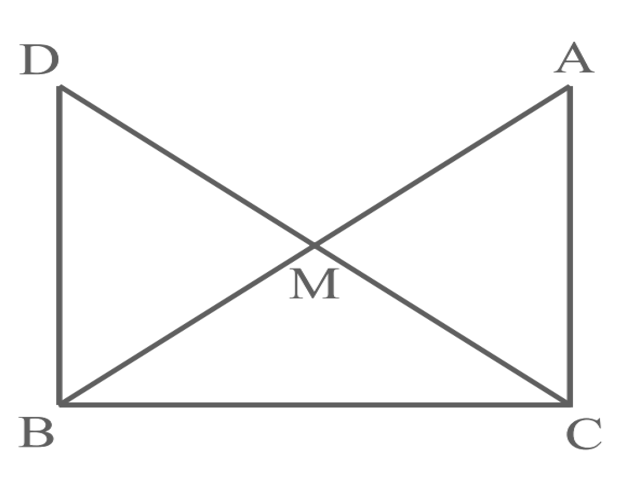
\includegraphics[width=\columnwidth]{figs/Screenshot.png}
  \caption{$\triangle \vec{ACB} ,\triangle \vec{DCB}$ with Mid-Point $\vec{M}$}
  \label{fig:triangles}
\end{figure}
\begin{enumerate}[label =(\roman*)]
	\item $\triangle \vec{AMC} \cong \triangle \vec{BMD}$
	\item $\angle \vec{DBC}$ is a right angle. 
	\item $\triangle \vec{DBC} \cong  \triangle \vec{ACB}$ 
	\item $\vec{CM} = \frac{1}{2} \vec{AB}$
\end{enumerate}
\pagebreak
\solution\\
\textbf{CONSTRUCTION STEPS :}
\begin{enumerate}
\item Let us Assume , the input parameters as ;
\begin{table}[H]
\centering
	\begin{tabular}{|c|c|c|}
\hline
\textbf{Parameter} & \textbf{Value} & \textbf{Description} \\
\hline
	$\vec{B}$ & $\myvec{0\\0}$ & Reference point at Origin \\
\hline
	$\vec{C}$ & $\myvec{6\\0}$ & point $\vec{C}$ on the same axis of $\vec{B}$ \\
\hline
    $l$ & $\norm{\vec{B}-\vec{C}}$ & Length of side  $\vec{BC}$ \\
\hline
\end{tabular}

	  \caption{Input Parameters}
	  \label{Table-1:Input_params}
\end{table}

\item the output can be calculated as ;
\begin{table}[H]
\centering
	\begin{tabular}{|c|c|p{5cm}|}
\hline
\textbf{Parameter} & \textbf{Value} & \textbf{Description} \\
\hline
	$\vec{C}$ & $\myvec{l\\0}$ & point $\vec{C}$ with length $l$ on the same axis of $\vec{B}$ \\
\hline
	$\vec{D}$ & $\myvec{0  \\ l }$ & $x = 0$ , $y = l$ i.e $x,y$ are co-ordinates of axes in XY-plane \\
\hline
	$\vec{A}$ & $\myvec{l \\ l }$ & $x = l$ , $y = l$ \\
 \hline
    $\vec{M}$ & $\brak{\frac{\vec{A+B}}{2}}$ & Mid-point of $\vec{AB}$ \\
\hline
\end{tabular}

	  \caption{Output Parameters}
	  \label{Table-2:Output_params}
\end{table}

		$\therefore$ By, Plotting these points we get the required Image \figref{fig:fig-2}

\begin{figure}[H]
	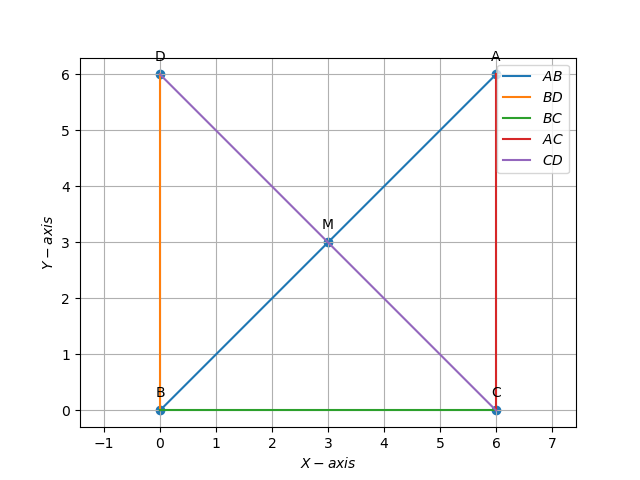
\includegraphics[width = \columnwidth]{figs/python_plot.png}
    \caption{PYTHON Plot of $\triangle \vec{ACB} ,\triangle \vec{DCB}$ with Mid-Point $\vec{M}$}
    \label{fig:fig-2}
\end{figure}
\end{enumerate}
\end{enumerate}
\end{document}
